The observation of neutrino oscillations~\cite{} has revealed limitations of the Standard Model. In particular, it demonstrated that lepton flavour is not a strictly conserved quantity in the neuttal lepton sector. 
Extending the Standard Model to include right-handed neutrinos naturally accommodated lepton flavour violation in the framework of quatum field theory. 
As a consequence, processes that violate lepton flavour in the charged lepton sector --- known as charged lepton flavour violation (cLFV) --- are also expected to occur at some level. 
\\
Examples of such processes include $\mu^+ \to e^+ + \gamma$ (searched for by the MEG experiment at PSI) and $\mu^+ \to e^+ e^- e^+$ (target of the MU3e experiemnt). 
Although no cLFV process has yet been observed, decades of experimental searches habe significalty imporved the upper limit on their brachnich ratios, as illustraded in Figure~\ref{fig:clfv_history}. 
These increasingly stringent limits provide valuable constraints on pyhscs beyond the Standard Model. 
\begin{figure}
    \centering
    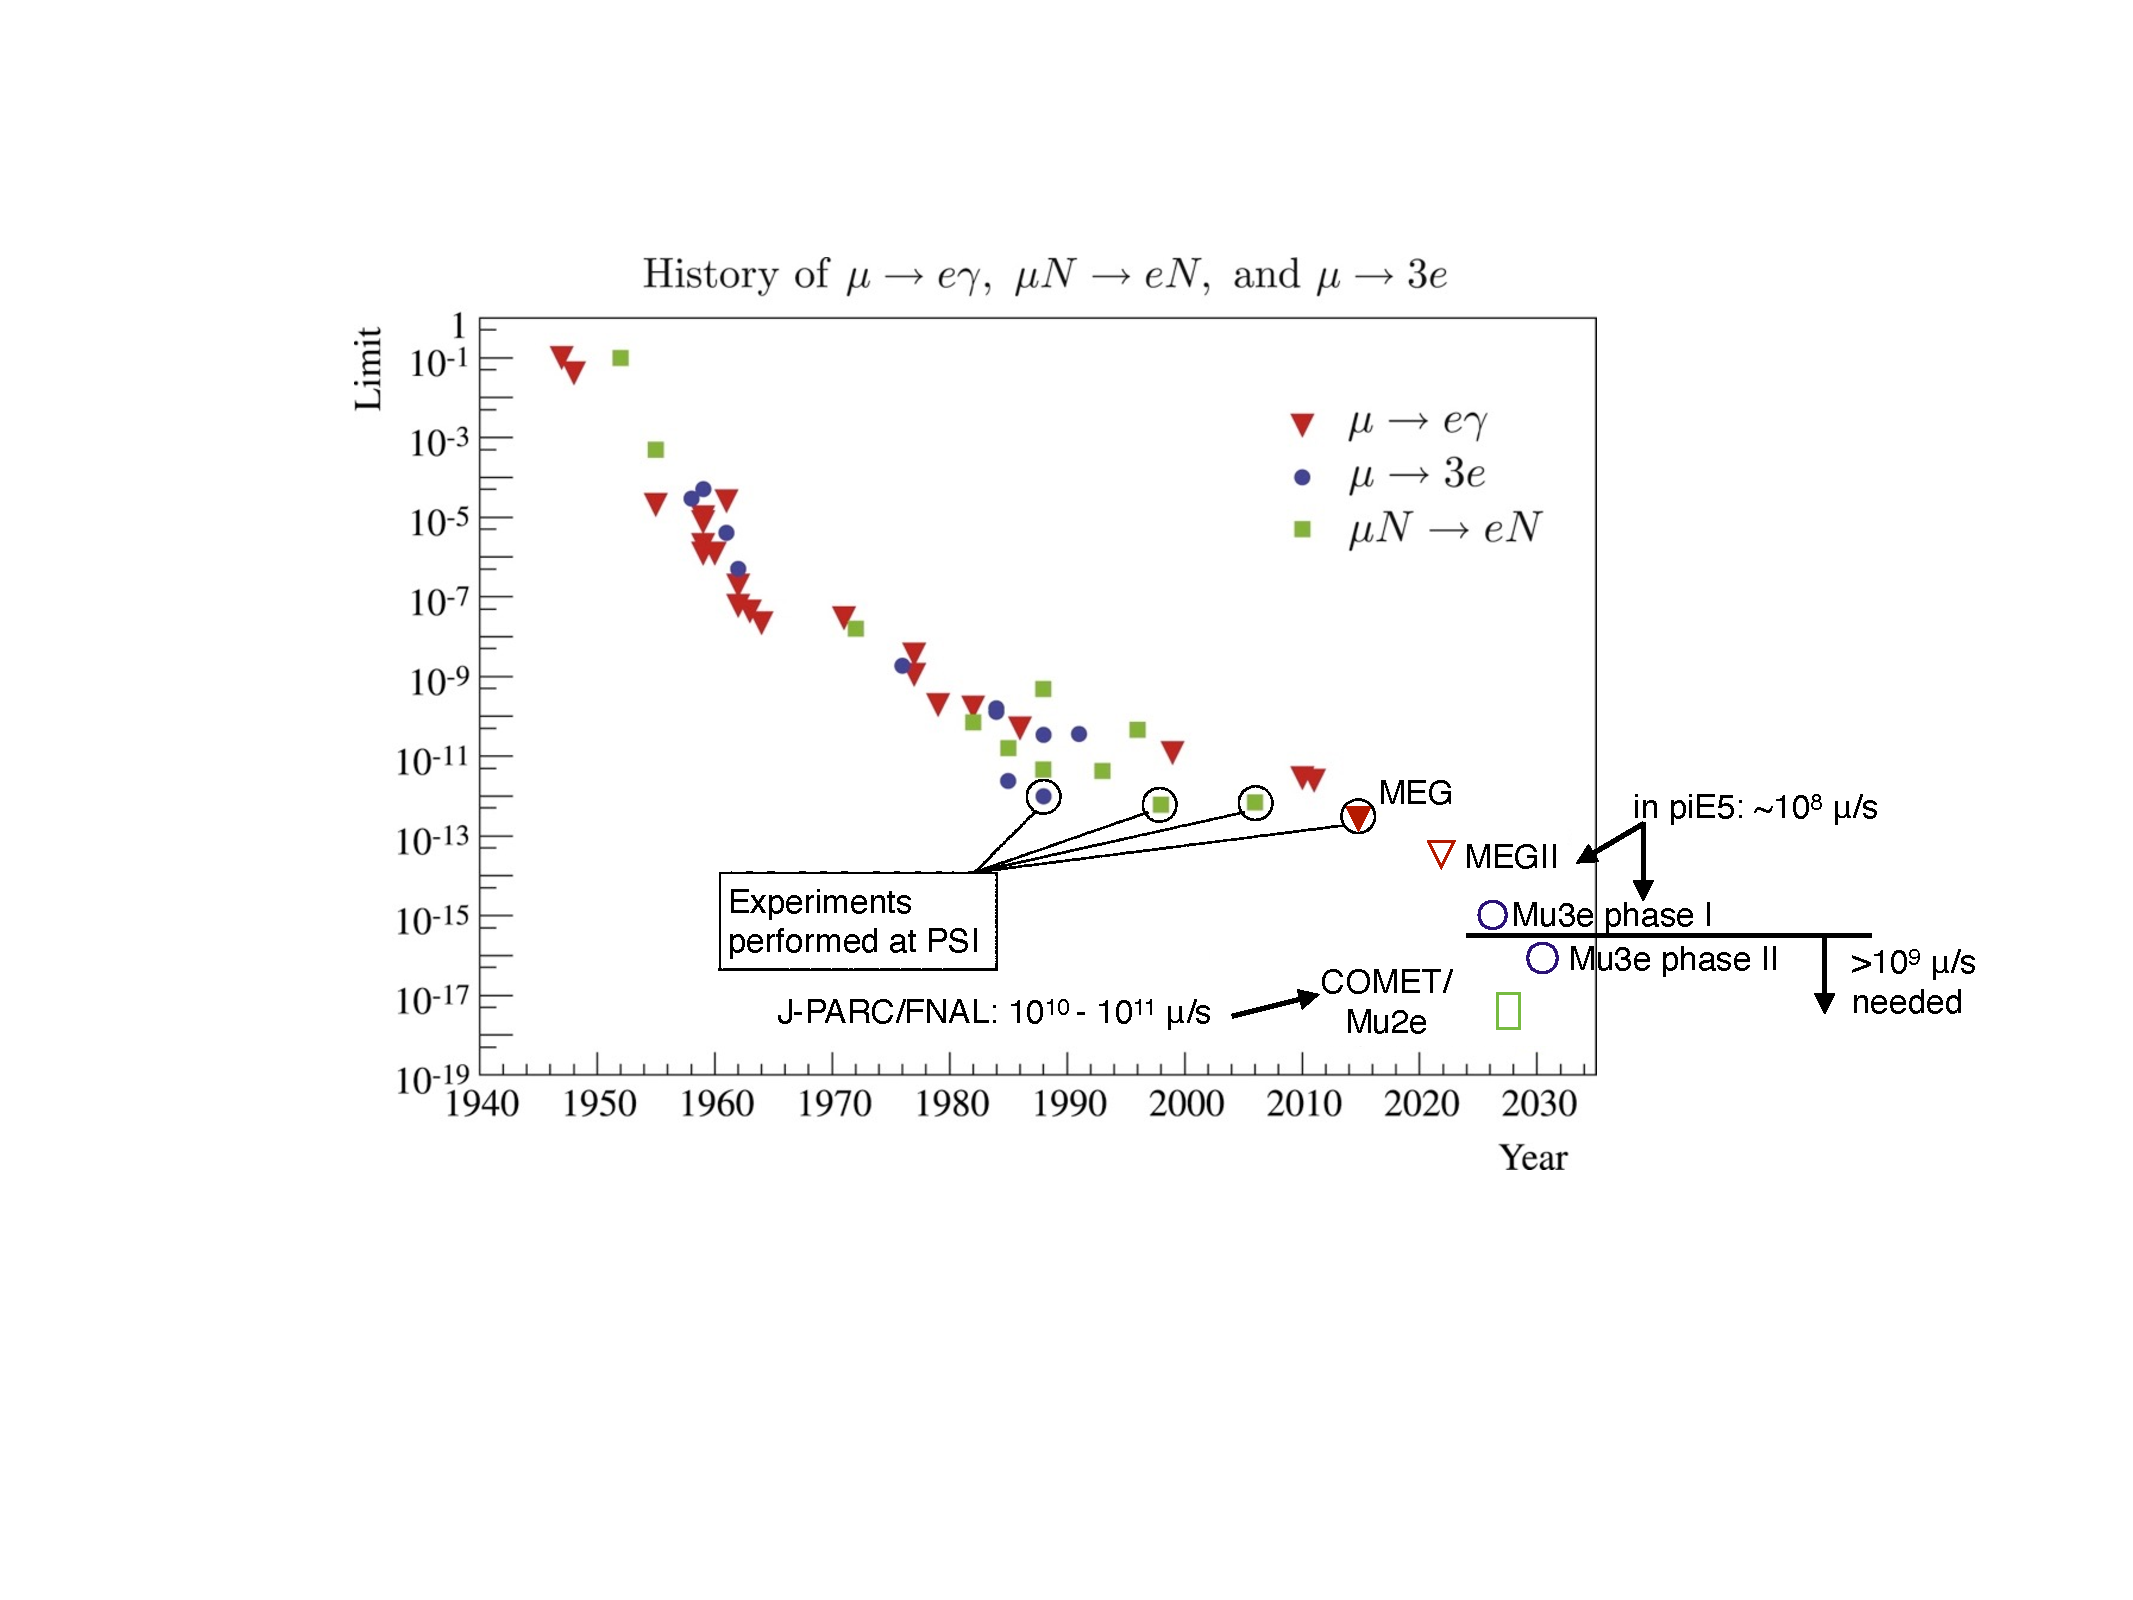
\includegraphics[width=0.8\textwidth]{figures/cLFV_history.pdf}
    \caption{History of the upper limits on the branching ratios of different cLFV processes~\cite{aiba2021science}.}\label{fig:clfv_history}
\end{figure}